% --------------------------------------------------------------------------------------------------
% SPDX-License-Identifier: Apache-2.0
% SPDX-FileCopyrightText: (C) 2021-2021, Jayesh Badwaik <jayesh@badwaik.dev>
% --------------------------------------------------------------------------------------------------
\makeatletter
\def\input@path{{./texmf}}
\makeatother
\documentclass[aspectratio=1610,10pt]{penchbeamer}
\title{Adapting Software Engineering Practices for Scientific Software}
\author[\textbf{Jayesh Badwaik}]{{Salem El Sayed, \textbf{Jayesh Badwaik}}
 }
 \institute[ ]{
  \url{https://go.fzj.de/jayesh-underse2023}
  \\[2ex]
  \url{https://github.com/jbadwaik/underse2023}
}
\date{September 28, 2023}

\usetheme{Boadilla}
\usecolortheme{pench}

\begin{document}
\maketitle


\begin{frame}
  \begin{center}
    \begin{huge}
      \textbf{Background}
    \end{huge}
  \end{center}
\end{frame}

\begin{frame}
  \frametitle{About Me}
  \begin{minipage}{0.4\textwidth}
    \begin{figure}
      \begin{center}
        
\includegraphics[width=0.8\textwidth]{static/jayesh.png}
      \end{center}
    \end{figure}
  \end{minipage}
  \begin{minipage}{0.45\textwidth}
    \begin{enumerate}
      \item In the HPC Domain since 2020.
      \item Worked on improving performance of applications on HPC systems
        through both accelerators and I/O systems.

      \item Currently part of the Accelerating Devices division at J\"ulich
        Supercomputing Centre, exploring programming models for accelerators.
    \end{enumerate}
    \textbf
    {"In theory, theory and practice are the same. In practice, they are not."}
  \end{minipage}
\end{frame}

\begin{frame}
  \begin{columns}
    \begin{column}{0.3\textwidth}
      \frametitle{{\small Dr.} Salem el Sayed}
      \begin{huge}
        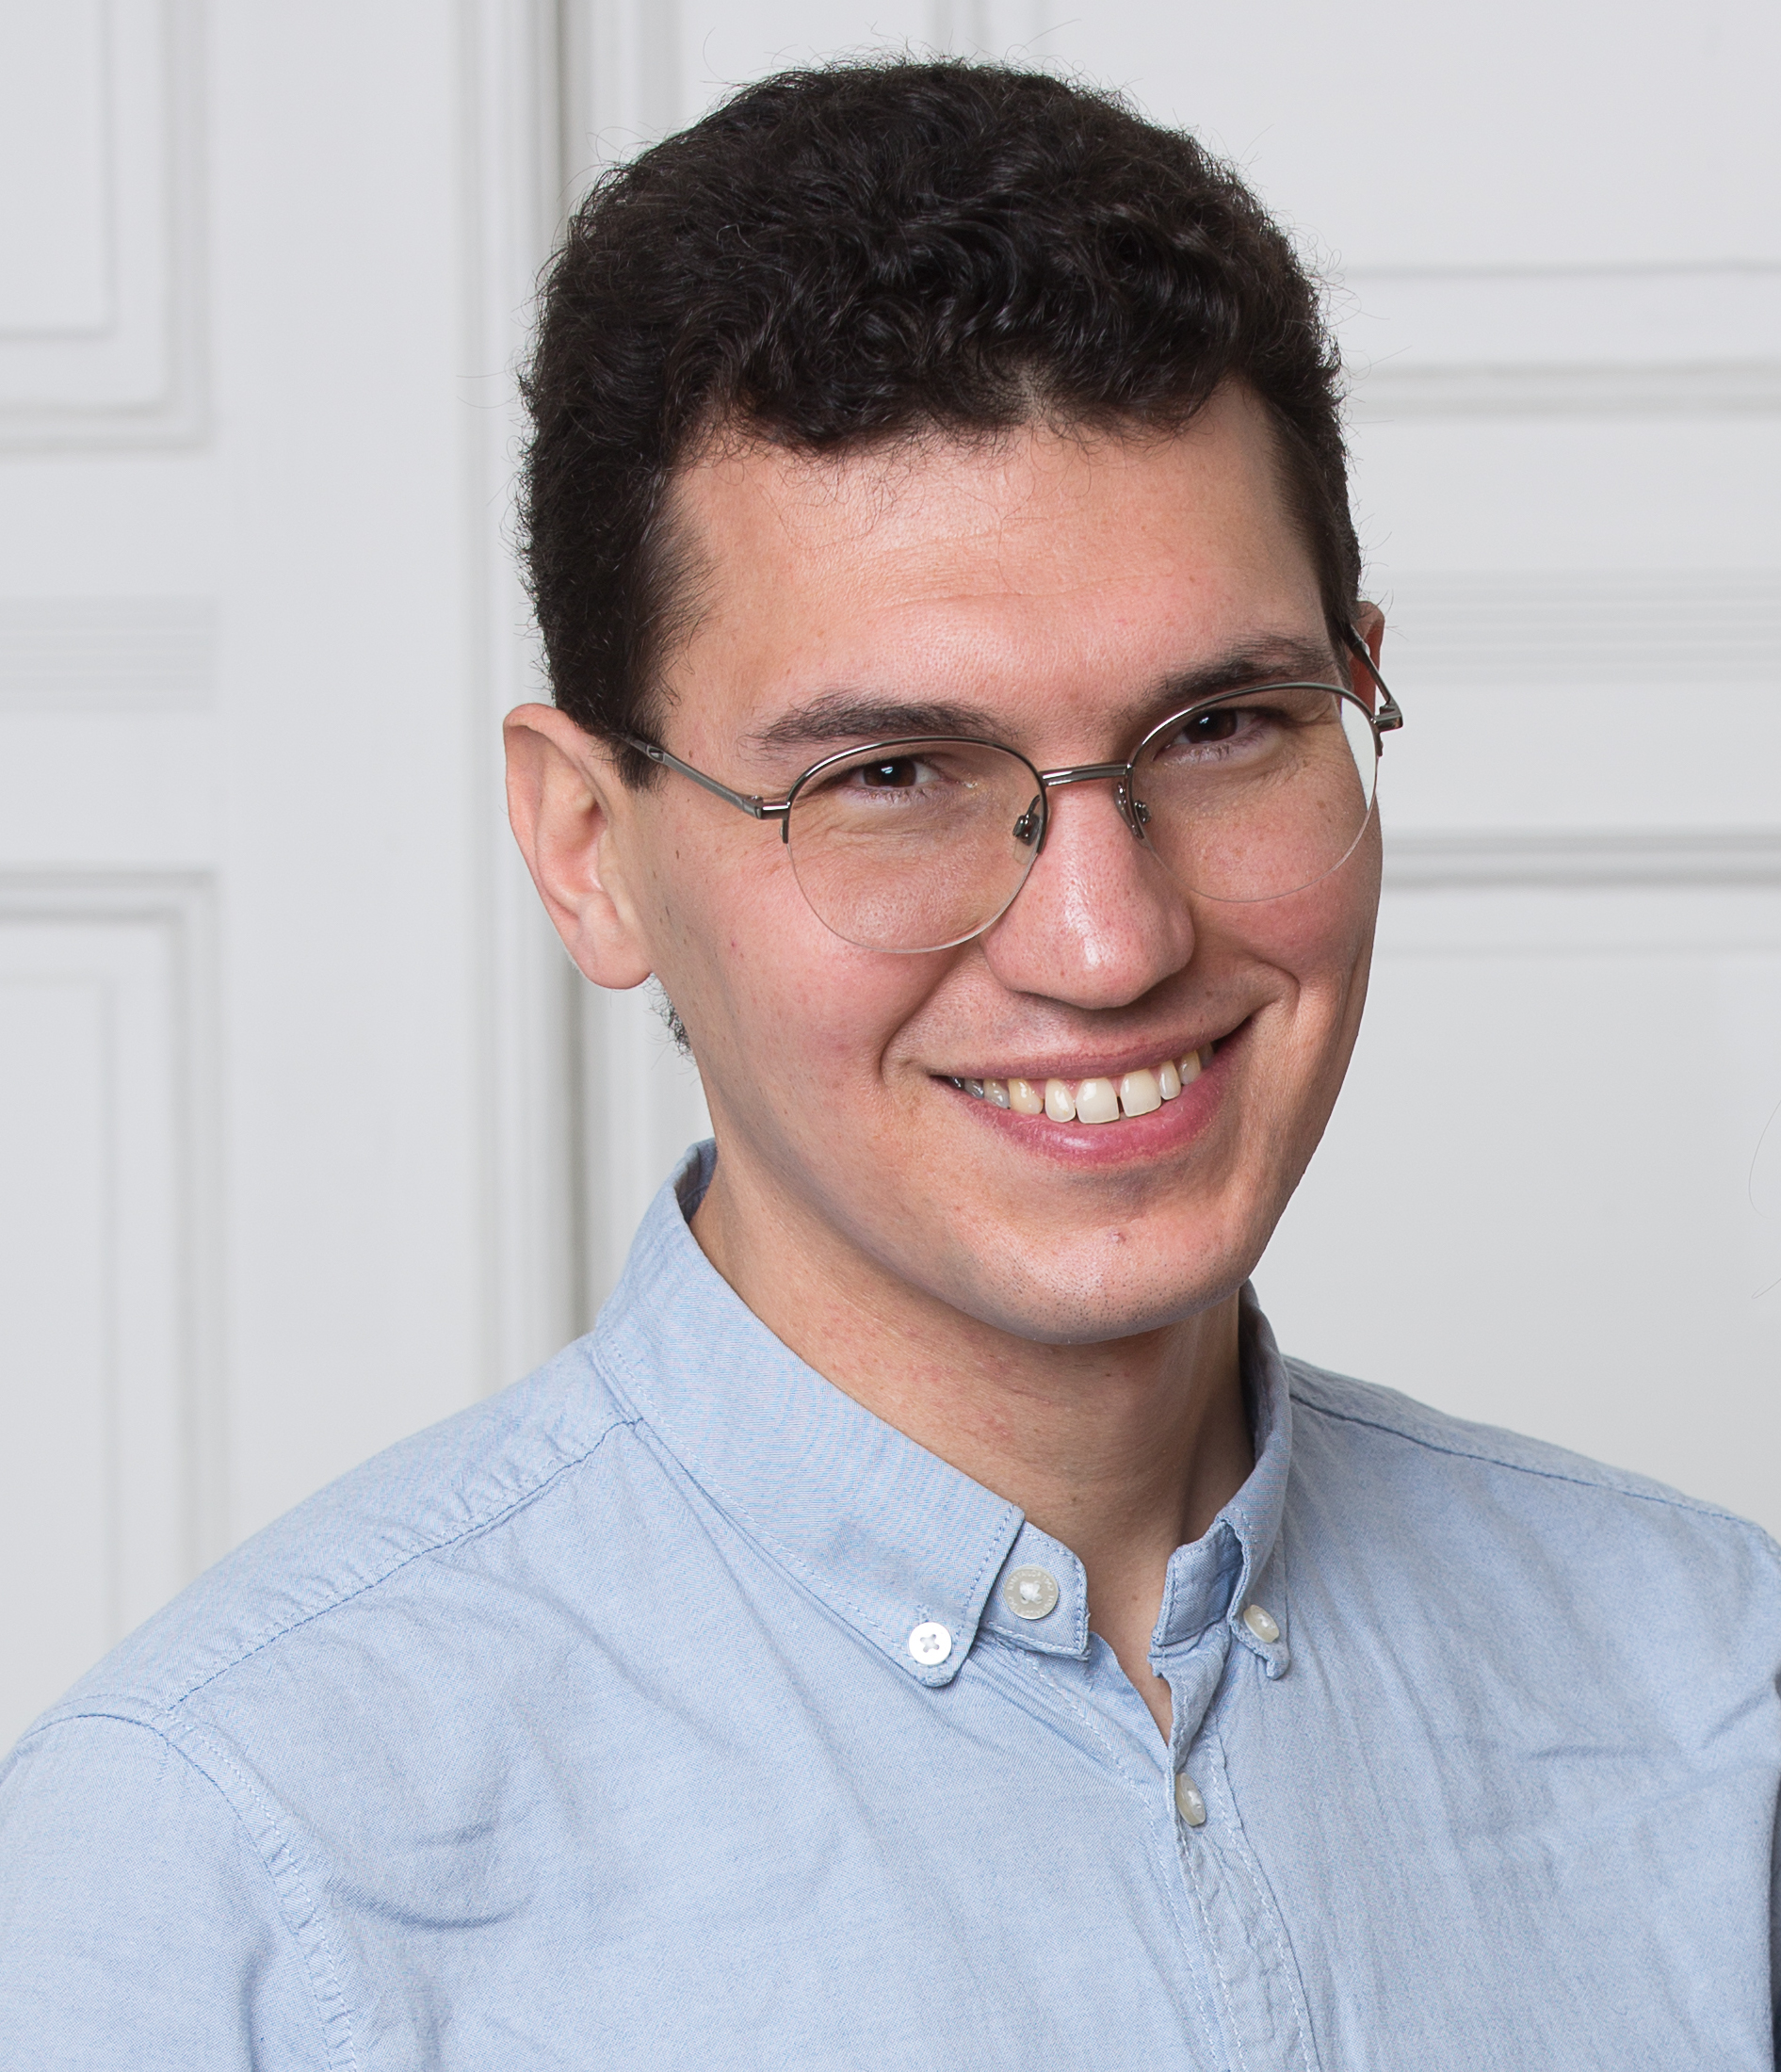
\includegraphics[scale=0.07]{images/SalemElSayed-Portrait.jpg}
      \end{huge}
    \end{column}
    \begin{column}{0.6\textwidth}
      \begin{enumerate}
        \item In the HPC domain since 2010.
        \item Dealt with bringing new tech to scientific codes in the context of many projects
        \item Since 2021 part of the \textit{HPCCDSS}\footnote{https://www.fz-juelich.de/en/ias/jsc/about-us/structure/divisions/high-performance-computing-cloud-and-data-systems-and-services-division} department in the JSC - which deals among others with procurring, deploying, testing and tuning of Juelich HPC and storage systems.
      \end{enumerate}
      \textbf{"If we make our systems better, but no one can use it, we are making them worse!"}
    \end{column}
  \end{columns}
\end{frame}



\begin{frame}
  \frametitle{Motivation}

  \begin{center}
    \begin{huge}
      \textbf{Acclerated Programming}
    \end{huge}
  \end{center}
\end{frame}

\begin{frame}
  \frametitle{Programming Models}
  \frametitle{Confidence in Ported / Generalized Code}


  \begin{minipage}{0.3\textwidth}
    \begin{figure}
      \begin{center}
        
\includegraphics[width=0.8\textwidth]{static/openmp.png}
      \end{center}
    \end{figure}
  \end{minipage}
  \begin{minipage}{0.3\textwidth}
    \begin{figure}
      \begin{center}
        
\includegraphics[width=0.8\textwidth]{static/cuda.png}
      \end{center}
    \end{figure}
  \end{minipage}
  \begin{minipage}{0.3\textwidth}
    \begin{figure}
      \begin{center}
        
\includegraphics[width=0.8\textwidth]{static/stdpar.png}
      \end{center}
    \end{figure}
  \end{minipage}

  \begin{minipage}{0.3\textwidth}
    \begin{figure}
      \begin{center}
        
\includegraphics[width=0.8\textwidth]{static/sycl.png}
      \end{center}
    \end{figure}
  \end{minipage}
  \begin{minipage}{0.3\textwidth}
    \begin{figure}
      \begin{center}
        
\includegraphics[width=0.8\textwidth]{static/graphcore.jpg}
      \end{center}
    \end{figure}
  \end{minipage}
  \begin{minipage}{0.3\textwidth}
    \begin{figure}
      \begin{center}
        
\includegraphics[width=0.8\textwidth]{static/opencl.png}
      \end{center}
    \end{figure}
  \end{minipage}
\end{frame}

\begin{frame}
  \frametitle{I/O Systems for Exascale Programming}

  \begin{figure}
    \begin{center}
      
\includegraphics[width=0.5\textwidth]{static/posix.png}
    \end{center}
  \end{figure}
  \vspace{2ex}

  \begin{center}
    \begin{large}
      \textbf{Alternatives Break Classical Assumptions}
    \end{large}
  \end{center}
  \begin{itemize}
    \item How to make it worthwhile for software to experiments with new I/O
      systems?
    \item How to have some guarantees that the experiments we do are close to
      real world use cases?
  \end{itemize}
\end{frame}


\begin{frame}
  \frametitle{3 Rs of Research Software Engineering}
  \framesubtitle{
  \href{https://hdsr.mitpress.mit.edu/pub/f0f7h5cu/release/2}{Promoting the 3Rs}}

  \begin{huge}
    \begin{itemize}
      \item Readability
      \item Resilience
      \item Reusability
    \end{itemize}
  \end{huge}

\end{frame}

\begin{frame}
  \frametitle{Goal of Today's Session}

  \begin{enumerate}
    \item Pain points in current workflows.
    \item List of topics to get things moving.
    \item Please bring up any topics that you feel.
  \end{enumerate}

  \textbf{Assumptions...}
  \begin{itemize}
    \item Users/Developers are interested in RSE
    \item Replace constraints of time with constraints of tools
      (I wouldn't have to do this if a reliable tool existed).
  \end{itemize}
  \vspace{2ex}

  \textbf{But, taking advantage of yesterday's session...}
\end{frame}


\begin{frame}
  \begin{figure}
    \begin{center}
      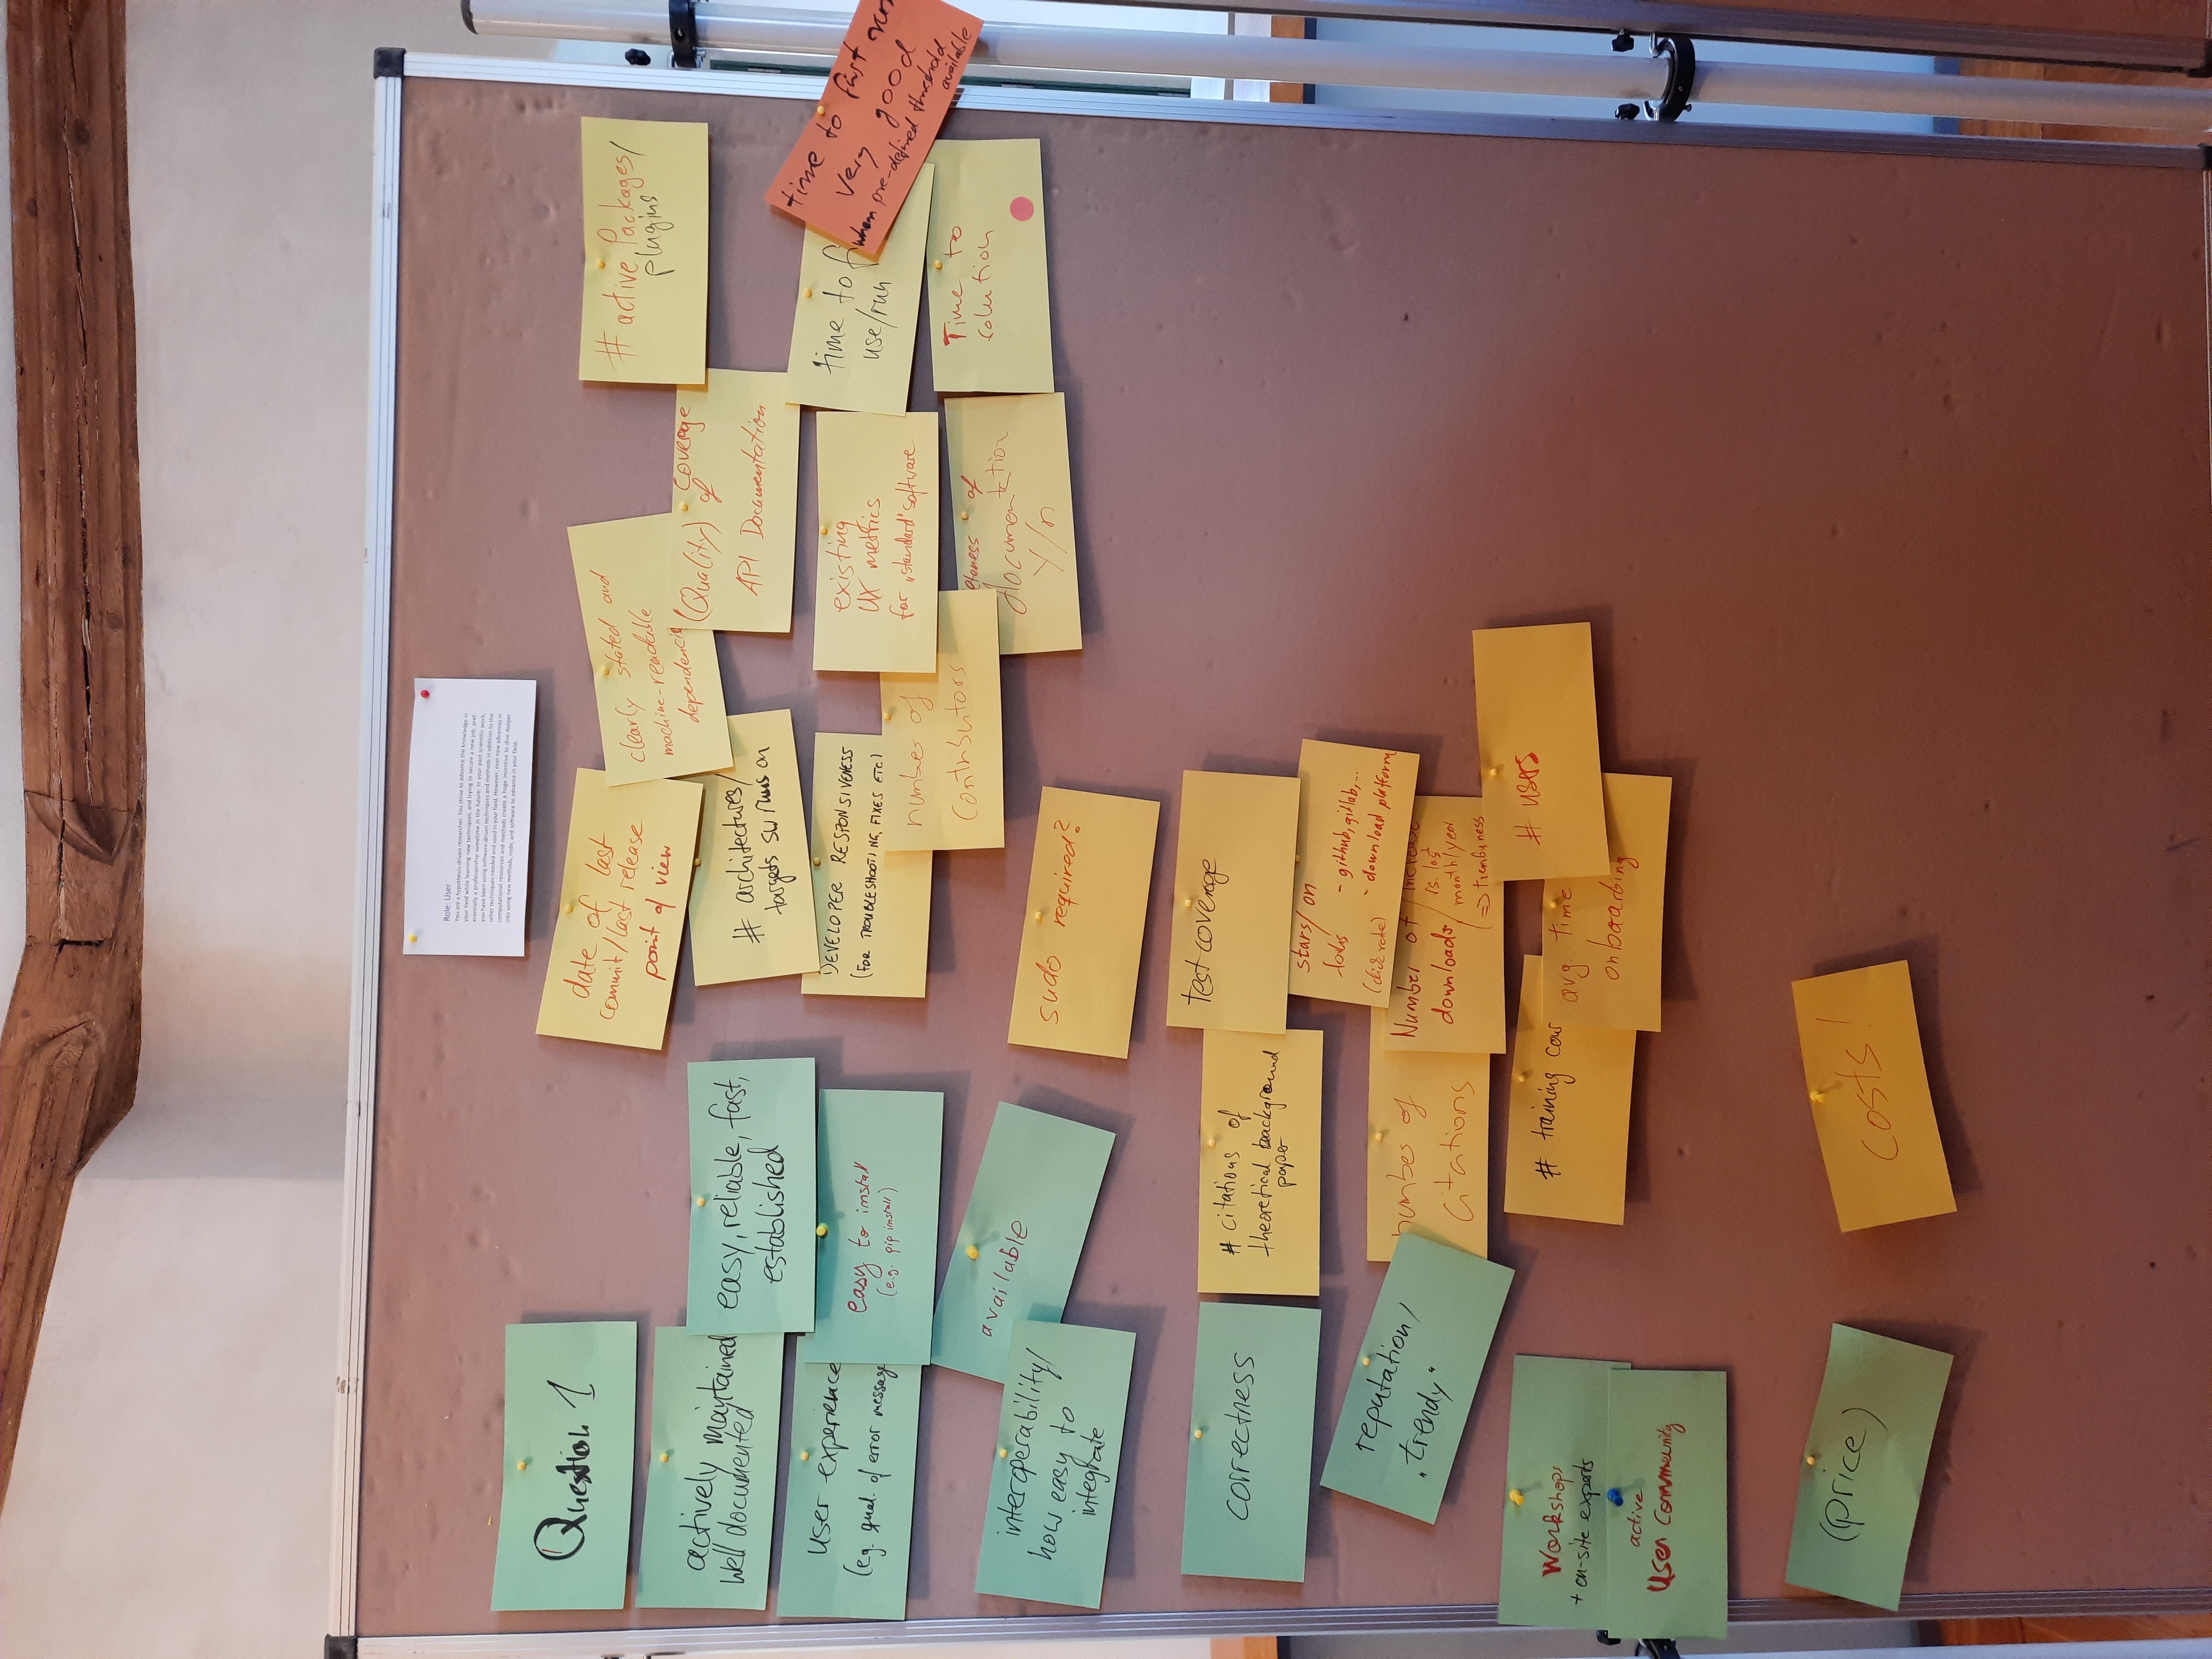
\includegraphics[height=0.8\textheight]{static/underse2023.png}
    \end{center}
  \end{figure}
\end{frame}

\begin{frame}
  \frametitle{Promise (Reliability)}

  \begin{itemize}
    \item Actively maintained, well documented code.
    \item Date of Last Commit
    \item Number of Architectures Supported (OS as well?)
    \item Number of Users
    \item Quality of Tests and API Documentation
    \item Repo Analytics like time to close issues, merge PRs
  \end{itemize}
\end{frame}

\begin{frame}
  \frametitle{Reusability}

  \begin{itemize}
    \item Ease of Integration
    \item Interoperability
    \item Easy to Install (\texttt{pip install} ?)
    \item \texttt{sudo} Required
    \item Clearly Stated and Machine Readable Dependencies
    \item Time to First Run
    \item Time to Solution
    \item Fast
    \item Availability in Package Managers
  \end{itemize}
\end{frame}

\begin{frame}
  \frametitle{Reliability}

  \begin{itemize}
    \item Correctness
    \item Reliable
    \item Established
    \item Test Coverage
    \item Reproducible
    \item Automatic Evaluation
    \item Comparative Benchmarks
  \end{itemize}
\end{frame}

\begin{frame}
  \frametitle{Resilience}
  \begin{itemize}
    \item Reputation
    \item Active User Community
    \item On-Site Experts
    \item Training Courses
    \item Developer Responsiveness
    \item Number of Contributors
    \item Quality of Error Messages
    \item Average Time Onboarding
  \end{itemize}

\end{frame}


\end{document}
